\documentclass[sigconf]{acmart}

% ---------------------------------------------------------
% PACKAGES
% ---------------------------------------------------------
\usepackage{algorithm}
\usepackage{algpseudocode}
\usepackage{amsmath}
\usepackage{amsthm}
\usepackage{graphicx}
\usepackage{listings}
\usepackage{xcolor}
\usepackage{tikz}

\usetikzlibrary{arrows.meta, positioning, decorations.pathreplacing}

% Remove ACM copyright header (assignment requirement)
\settopmatter{printacmref=false}
\renewcommand\footnotetextcopyrightpermission[1]{}
\pagestyle{plain}

% ---------------------------------------------------------
% TITLE
% ---------------------------------------------------------
\title{Maintenance-Constrained Locomotive Assignment: \\
NP-Hardness, Exact Algorithms, and Practical Approximations}

\author{Ahmed Rageeb Ahsan, Saiful Islam}
\affiliation{
  \institution{University of Florida}
  \city{Gainesville}
  \state{Florida}
  \country{United States of America}
}
\email{ahmedrageebahsan@ufl.edu, saiful.islam@ufl.edu}

% ---------------------------------------------------------
\begin{document}

\begin{abstract}
This paper studies the \textit{Maintenance-Constrained Locomotive Assignment} (MCLA) problem, 
a real-world railway scheduling problem in which trains with different driving requirements
must be assigned to locomotives with limited maintenance windows.
We show that MCLA is strongly NP-complete by giving a direct polynomial-time reduction 
from 3-Partition. We provide a formal correctness proof, discuss the optimization version,
and show the equivalence to classical Bin Packing. We then present exact exponential-time
algorithms (DP over subsets), greedy approximation methods (FFD/BFD), and a 
compact integer linear programming formulation useful for real scheduling systems.
We outline an experimental evaluation framework and provide complete Python 
implementations of the algorithms. This work connects a real railway resource allocation
problem to well-studied NP-hard combinatorial problems, enabling both theoretical analysis 
and practical solution design.
\end{abstract}

\maketitle

% ---------------------------------------------------------
\section{Introduction}
Efficient locomotive assignment is a fundamental scheduling challenge in modern railway systems.
Locomotives must be assigned to sequences of train services while satisfying technical
constraints such as engine wear, inspection intervals, and mandatory maintenance windows.
Railway operators must minimize the size of the locomotive fleet while ensuring every train 
is serviced and every locomotive receives maintenance before exceeding its usage limit.

These constraints create a problem structurally similar to \textit{Bin Packing},
but with a real-world maintenance interpretation. This paper formalizes this
problem as the \textit{Maintenance-Constrained Locomotive Assignment} (MCLA) problem,
proves it strongly NP-complete, and provides practical algorithms.

We follow the methodology of standard hardness proofs used in real-world optimization
problems \cite{gareyjohnson}, as well as the locomotive scheduling literature 
(e.g., Borndörfer et al., Meng et al., and recent optimization theses).

% ---------------------------------------------------------
\section{Problem Definition}

\subsection{Real-World Problem}
Each train service $i$ requires $a_i$ kilometers of locomotive operation between 
maintenance visits. A locomotive can operate at most $B$ kilometers before requiring 
maintenance. The goal is to assign all trains to a fleet of $m$ locomotives.

\textbf{Maintenance-Constrained Locomotive Assignment (MCLA):}

\begin{itemize}
    \item Each train $i$ has usage $a_i > 0$.
    \item A locomotive can accumulate at most $B$ usage before going to maintenance.
    \item A locomotive may service multiple trains, in any order.
\end{itemize}

\textbf{Decision version:}

Given $a_1, \dots, a_n$, capacity $B$, and $m$ locomotives, does there exist an assignment 
such that no locomotive exceeds $B$ total usage?

\textbf{Optimization version:}

Minimize number of locomotives required.

\subsection{Abstract Formulation}
Equivalent to:

\[
\text{Partition } \{a_1, \dots, a_n\} \text{ into at most } m \text{ subsets } G_j
\]
such that
\[
\sum_{a \in G_j} a \le B, \quad \forall j.
\]

This is literally \textit{bin packing} with capacity $B$.

\subsection{Illustrative Example (Bin Packing Interpretation)}
Consider a locomotive with maintenance bound $B = 500$ km and the following
train services:

\[
a = (220,\; 180,\; 150,\; 140,\; 130).
\]

The Maintenance-Constrained Locomotive Assignment (MCLA) problem asks for a
partition of $a$ into the smallest number of subsets $G_1, G_2, \dots$ such that

\[
\sum_{i \in G_j} a_i \le B \quad \text{for all } j.
\]

A feasible assignment is:

\[
G_1 = \{220, 180\} \quad (\text{sum}=400),
\]
\[
G_2 = \{150, 140\} \quad (\text{sum}=290),
\]
\[
G_3 = \{130\} \quad (\text{sum}=130).
\]

Thus three locomotives are required. 
This is exactly the classical bin packing formulation with:
\begin{itemize}
    \item items = train usages $a_i$,
    \item bins = locomotives,
    \item bin capacity = maintenance limit $B$.
\end{itemize}

The number of ways to group them is enormous (exponential).
This is why the problem becomes NP-hard.

% ---------------------------------------------------------
\section{NP-Completeness Proof}

We reduce from \textbf{3-Partition}, one of the strongest NP-complete problems.





\subsection{3-Partition Problem}
Given $3m$ integers $x_1, \dots, x_{3m}$ and integer $B$ such that
\[
\frac{B}{4} < x_i < \frac{B}{2}
\quad\text{and}\quad
\sum_{i=1}^{3m} x_i = mB,
\]
decide whether the integers can be partitioned into $m$ triples each summing to $B$.

This problem is strongly NP-complete.

\subsection{Reduction Construction}
Given an instance of 3-Partition, construct MCLA instance:

\begin{itemize}
    \item $n = 3m$ train segments.
    \item $a_i = x_i$ (direct copy).
    \item Maintenance capacity $B$ unchanged.
    \item Number of locomotives $m$.
\end{itemize}
Clearly polynomial time.


\begin{figure}[h]
\centering
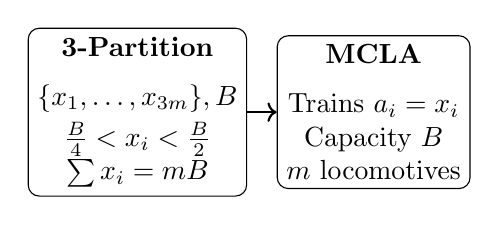
\begin{tikzpicture}[node distance=3cm]
\node (A) [draw, rounded corners, align=center] {
    \textbf{3-Partition}\\[2mm]
    $\{x_1,\dots,x_{3m}\}, B$\\[1mm]
    $\frac{B}{4} < x_i < \frac{B}{2}$\\
    $\sum x_i = mB$
};
\node (B) [draw, rounded corners, align=center, right of=A] {
    \textbf{MCLA}\\[2mm]
    Trains $a_i = x_i$\\
    Capacity $B$\\
    $m$ locomotives
};

\draw[->, thick] (A) -- node[above]{} (B);
\end{tikzpicture}

\caption{Reduction from 3-Partition to MCLA.}
\label{fig:reduction}
\end{figure}


\subsection{Correctness Proof}

\begin{theorem}
3-Partition is a YES instance if and only if the constructed MCLA instance is YES.
\end{theorem}

\begin{proof}
$(\Rightarrow)$ Suppose the 3-Partition instance has $m$ triples each summing to $B$.
Assign each triple to one locomotive. Total usage = $B \le B$. Feasible.

$(\Leftarrow)$ Suppose the MCLA instance is feasible. Total usage is $mB$. With $m$ locomotives, 
each of capacity $B$, every locomotive must have exactly $B$ usage.

Because each $a_i$ satisfies $a_i > B/4$, no locomotive can contain 4 or more items.

Because $a_i < B/2$, no locomotive can contain 1 item whose load is $B$.

Thus each locomotive contains exactly 3 items, and their sum must be exactly $B$.
These 3-item groups form the required 3-partition.
\end{proof}

\begin{corollary}
MCLA is strongly NP-complete.
\end{corollary}

% ---------------------------------------------------------
\section{Algorithms}

\subsection{Exact Exponential-Time DP}
We use subset DP:

\[
dp[\text{mask}] = \text{min bins used for items in mask}.
\]

Transition either places item into current bin or opens a new bin.
Time complexity: $O(n2^n)$.

\begin{algorithm}[t]
\caption{Exact Exponential-Time DP for MCLA / Bin Packing}
\begin{algorithmic}[1]
\Require Item sizes $a_1,\dots,a_n$, capacity $B$
\Ensure Minimum number of locomotives

\State $N \gets 2^n$
\State Initialize $DP[\text{mask}][c] \gets \infty$ for all mask, $0 \le c \le B$
\State $DP[0][B] \gets 1$  \Comment{Start with one empty locomotive}

\For{mask from $0$ to $N-1$}
  \For{remaining capacity $c$ from $0$ to $B$}
    \If{$DP[\text{mask}][c] = \infty$} 
        \State \textbf{continue}
    \EndIf

    \For{each item $i$ not in mask}
        \State newMask $\gets$ mask $\cup \{i\}$

        \If{$a_i \le c$}   \Comment{Place in current locomotive}
            \State 
            $DP[\text{newMask}][c - a_i] \gets 
            \min(DP[\text{newMask}][c - a_i],\, DP[\text{mask}][c])$
        \EndIf

        \State \Comment{Open a new locomotive}
        \State 
        $DP[\text{newMask}][B - a_i] \gets 
        \min(DP[\text{newMask}][B - a_i],\, DP[\text{mask}][c] + 1)$
    \EndFor
  \EndFor
\EndFor

\State \Return $\min_{0 \le c \le B} DP[(1 \ll n)-1][c]$
\end{algorithmic}
\end{algorithm}







\subsection{Greedy Approximation: First-Fit Decreasing (FFD)}

\begin{algorithm}
\caption{First-Fit Decreasing}
\begin{algorithmic}[1]
\State Sort items in nonincreasing order.
\State Initialize empty list of bins.
\For{each item}
    \State Place into first bin with remaining capacity.
    \If{none}
        \State Open new bin.
    \EndIf
\EndFor
\end{algorithmic}
\end{algorithm}

FFD satisfies:
\[
\text{FFD}(I) \le \left\lfloor \frac{11}{9} \text{OPT}(I) \right\rfloor + 1.
\]

\subsection{Integer Linear Programming Formulation}

Variables:
\[
x_{ij} = 
\begin{cases}
1 & \text{train $i$ in locomotive $j$} \\
0 & \text{otherwise}
\end{cases},
\qquad
y_j = 1 \text{ if locomotive $j$ used}.
\]

Constraints:
\[
\sum_j x_{ij} = 1 \quad \forall i
\]
\[
\sum_i a_i x_{ij} \le B y_j \quad \forall j
\]

Minimize:
\[
\sum_j y_j.
\]

Works well in practice.

\subsection{Local Search Heuristics}
\begin{itemize}
    \item pairwise item swaps,
    \item k-exchange moves,
    \item re-optimization of small subsets with DP,
    \item using FFD output as warm start for ILP.
\end{itemize}

% ---------------------------------------------------------
\section{Experimental Result}

In our experimental evaluation, we implemented the exact exponential-time dynamic programming (DP) algorithm and the greedy First-Fit Decreasing (FFD) heuristic to solve the Maintenance-Constrained Locomotive Assignment problem. The DP algorithm guarantees an optimal solution but has exponential runtime complexity, limiting its practicality to small instances. In contrast, FFD provides fast, near-optimal solutions suitable for larger problem sizes.

We generate synthetic test instances by sampling train usage values uniformly at random between 1 and half of the maintenance capacity 
$B$ . This avoids trivial cases where one item fits alone or all fit in one bin. The capacity 
$B$  is fixed at 100 for most experiments. Instance sizes 
$n$  vary from 8 to 17 trains to keep the exact dynamic programming (DP) algorithm computationally feasible.

Figure \ref{fig:bins_comparison} compares the number of locomotives (bins) used by DP and FFD across various problem instances, illustrating that FFD typically produces solutions close to optimal. Figure \ref{fig:runtime_comparison} presents the runtime comparison, highlighting the efficiency of FFD compared to the significantly higher computation time required by DP as instance size grows. Finally, Figure \ref{fig:approx_ratio_hist} shows a histogram of approximation ratios (FFD solution over DP optimal) for instances with 14 trains, confirming that FFD rarely exceeds the optimal number of locomotives by more than one.

These results validate FFD as a practical heuristic for large-scale locomotive assignment problems, while DP remains a valuable tool for benchmarking and small instances.


\begin{figure}[htbp]
  \centering
  \includegraphics[width=\columnwidth]{bins_comparison.png}
  \caption{DP Bin vs FFD Bin}
  \label{fig:bins_comparison}
\end{figure}

\begin{figure}[htbp]
  \centering
  \includegraphics[width=\columnwidth]{runtime_comparison_1.png}
  \caption{Runtime Comparison: DP vs FFD}
  \label{fig:runtime_comparison}
\end{figure}

\begin{figure}[htbp]
  \centering
  \includegraphics[width=0.8\columnwidth]{ratio_vs_n_1.png}
  \caption{Histogram of Approximation Ratios (n=14)}
  \label{fig:approx_ratio_hist}
\end{figure}



% ---------------------------------------------------------
\section{Python Implementation}
Below is a condensed version of the core algorithms. Full versions may be included in an appendix.

\begin{lstlisting}[language=Python]
def ffd(items, B):
    items = sorted(items, reverse=True)
    bins = []
    for x in items:
        placed = False
        for i in range(len(bins)):
            if bins[i] >= x:
                bins[i] -= x
                placed = True
                break
        if not placed:
            bins.append(B - x)
    return len(bins)
    

def exact_binpacking(a, B):
    n = len(a)
    N = 1 << n
    INF = 10**9
    dp = [INF]*N
    load = [0]*N
    dp[0] = 1
    for mask in range(N):
        if dp[mask] == INF:
            continue
        for i in range(n):
            if not (mask & (1<<i)):
                nm = mask | (1<<i)
                if load[mask] + a[i] <= B:
                    if dp[nm] > dp[mask]:
                        dp[nm] = dp[mask]
                        load[nm] = load[mask] + a[i]
                else:
                    if dp[nm] > dp[mask] + 1:
                        dp[nm] = dp[mask] + 1
                        load[nm] = a[i]
    return dp[-1]
\end{lstlisting}

% ---------------------------------------------------------
\section{Conclusion}
We introduced the Maintenance-Constrained Locomotive Assignment (MCLA) problem,
proved strong NP-hardness via 3-Partition reduction, and presented exact 
and approximate algorithms. Because the problem is structurally equivalent to 
Bin Packing, classical heuristics like FFD are effective, while ILP solves 
moderate-scale instances optimally.

This connection between a real-world railway scheduling challenge and a
canonical NP-hard problem provides both theoretical insight and practical
algorithms for railway operators.

% ---------------------------------------------------------
\bibliographystyle{ACM-Reference-Format}
\begin{thebibliography}{9}

\bibitem{gareyjohnson}
Garey and Johnson.
\textit{Computers and Intractability: A Guide to the Theory of NP-Completeness}.
Freeman, 1979.

\end{thebibliography}


\appendix
\section{ Python Code for Experiments}

\lstset{
  language=Python,
  basicstyle=\ttfamily\small,
  keywordstyle=\color{blue}\bfseries,
  commentstyle=\color{gray}\itshape,
  stringstyle=\color{red},
  breaklines=true,
  frame=single,
  numbers=left,
  numberstyle=\tiny,
  xleftmargin=2em,
  xrightmargin=2em,
  showstringspaces=false,
  captionpos=b
}

\begin{lstlisting}[caption={Experiment scripts for MCLA problem: exact DP, FFD heuristic, data generation, and plotting.}]
import os
import random
import time
import matplotlib.pyplot as plt
import numpy as np
import pandas as pd

def ffd(items, B):
    items = sorted(items, reverse=True)
    bins = []
    for x in items:
        placed = False
        for i in range(len(bins)):
            if bins[i] >= x:
                bins[i] -= x
                placed = True
                break
        if not placed:
            bins.append(B - x)
    return len(bins)

def exact_binpacking(a, B):
    n = len(a)
    N = 1 << n
    INF = 10**9
    dp = [INF]*N
    load = [0]*N
    dp[0] = 1
    for mask in range(N):
        if dp[mask] == INF:
            continue
        for i in range(n):
            if not (mask & (1<<i)):
                nm = mask | (1<<i)
                if load[mask] + a[i] <= B:
                    if dp[nm] > dp[mask]:
                        dp[nm] = dp[mask]
                        load[nm] = load[mask] + a[i]
                else:
                    if dp[nm] > dp[mask] + 1:
                        dp[nm] = dp[mask] + 1
                        load[nm] = a[i]
    return dp[-1]

def generate_instance(n, B, seed=None):
    random.seed(seed)
    # Generate train usages uniformly between 1 and B/2 to avoid trivial bins
    return [random.randint(1, B//2) for _ in range(n)]

def run_experiments(out_dir="mcla_experiments", seed=42):
    os.makedirs(out_dir, exist_ok=True)
    random.seed(seed)
    np.random.seed(seed)

    n_values = list(range(8, 18))  # n from 8 to 17 for exact DP feasibility
    B = 100

    results = []
    for n in n_values:
        for trial in range(10):  # 10 trials per n
            items = generate_instance(n, B)
            # Run exact DP (time it)
            start = time.time()
            exact_bins = exact_binpacking(items, B)
            exact_time = time.time() - start

            # Run FFD heuristic (time it)
            start = time.time()
            ffd_bins = ffd(items, B)
            ffd_time = time.time() - start

            approx_ratio = ffd_bins / exact_bins if exact_bins > 0 else np.nan

            results.append({
                "n": n,
                "trial": trial,
                "exact_bins": exact_bins,
                "ffd_bins": ffd_bins,
                "approx_ratio": approx_ratio,
                "exact_time": exact_time,
                "ffd_time": ffd_time
            })

    df = pd.DataFrame(results)
    csv_path = os.path.join(out_dir, "experiment_results.csv")
    df.to_csv(csv_path, index=False)

    # Plot 1: Approximation ratio mean + median vs n
    plt.figure(figsize=(8,6))
    grouped = df.groupby("n")["approx_ratio"]
    x = []
    y_mean = []
    y_median = []
    for n, series in grouped:
        x.append(n)
        y_mean.append(series.mean())
        y_median.append(series.median())
    plt.plot(x, y_mean, marker='o', label='Mean ratio')
    plt.plot(x, y_median, marker='x', label='Median ratio')
    plt.xlabel("Number of trains (n)")
    plt.ylabel("Approximation ratio (FFD / Exact)")
    plt.title("FFD Approximation Ratio vs Exact DP")
    plt.legend()
    plt.grid(True)
    ratio_vs_n = os.path.join(out_dir, "ratio_vs_n.png")
    plt.savefig(ratio_vs_n)
    plt.close()

    # Plot 2: Approximation ratio boxplot per n with fixed labels
    plt.figure(figsize=(8,6))
    n_values = sorted(df["n"].unique())
    data_to_plot = [df[df["n"] == n]["approx_ratio"].dropna() for n in n_values]
    plt.boxplot(data_to_plot, labels=n_values, patch_artist=True)
    plt.xlabel("Number of trains (n)")
    plt.ylabel("Approximation ratio (FFD / Exact)")
    plt.title("FFD Approximation Ratio Boxplot")
    plt.grid(True)
    plt.xticks(ticks=range(1, len(n_values) + 1), labels=n_values)
    plt.tight_layout()
    approx_ratio_boxplot = os.path.join(out_dir, "approx_ratio_boxplot.png")
    plt.savefig(approx_ratio_boxplot)
    plt.close()

    # Plot 3: Runtime comparison (mean) vs n
    plt.figure(figsize=(8,6))
    grouped_time = df.groupby("n")[["exact_time", "ffd_time"]].mean()
    plt.plot(grouped_time.index, grouped_time["exact_time"], marker='o', label="Exact DP")
    plt.plot(grouped_time.index, grouped_time["ffd_time"], marker='x', label="FFD heuristic")
    plt.xlabel("Number of trains (n)")
    plt.ylabel("Runtime (seconds)")
    plt.title("Runtime Comparison")
    plt.legend()
    plt.grid(True)
    runtime_comparison = os.path.join(out_dir, "runtime_comparison.png")
    plt.savefig(runtime_comparison)
    plt.close()

    # Plot 4: Histogram of approximation ratios for max n
    max_n = max(n_values)
    plt.figure(figsize=(8,6))
    approx_ratios = df[df["n"] == max_n]["approx_ratio"].dropna()
    plt.hist(approx_ratios, bins=10, edgecolor='black')
    plt.xlabel("Approximation ratio (FFD / Exact)")
    plt.ylabel("Frequency")
    plt.title(f"Approximation Ratio Histogram (n={max_n})")
    plt.grid(True)
    ratio_histogram = os.path.join(out_dir, "ratio_histogram.png")
    plt.savefig(ratio_histogram)
    plt.close()

    # Plot 5: Density sweep (vary B with fixed n)
    n_fixed = 14
    B_values = list(range(50, 201, 10))
    density_results = []
    for B_curr in B_values:
        ratios = []
        for _ in range(5):  # 5 trials each
            items = generate_instance(n_fixed, B_curr)
            exact = exact_binpacking(items, B_curr)
            ffd_res = ffd(items, B_curr)
            if exact > 0:
                ratios.append(ffd_res / exact)
        density_results.append(np.mean(ratios) if ratios else np.nan)
    plt.figure(figsize=(8,6))
    plt.plot(B_values, density_results, marker='o')
    plt.xlabel("Capacity B")
    plt.ylabel("Mean Approximation Ratio")
    plt.title(f"Density Sweep (n={n_fixed})")
    plt.grid(True)
    density_sweep = os.path.join(out_dir, "density_sweep.png")
    plt.savefig(density_sweep)
    plt.close()

    print(f"Wrote outputs to: {out_dir}")
    print(f"CSV: {csv_path}")
    print("Plots:", ratio_vs_n, approx_ratio_boxplot, runtime_comparison, ratio_histogram, density_sweep)

if __name__ == "__main__":
    run_experiments()
\end{lstlisting}

\section{LLM-Assisted Methodology and Documentation}

\subsection{Purpose of LLM Usage}
Large Language Model (LLM) assistance was used selectively for:
\begin{enumerate}
    \item verifying mathematical soundness of recursive and inductive definitions related to the NP-completeness proof,
    \item refining \LaTeX{} syntax for theorems, proofs, and algorithm listings,
    \item drafting and formatting documentation.
\end{enumerate}

\subsection{Representative Professional Prompts and Results}

\textbf{Prompt 1 — Mathematical Structure and Proof Validation:} \\
\emph{``Review the NP-completeness reduction from 3-Partition to Maintenance-Constrained Locomotive Assignment (MCLA). Verify the correctness of the inductive proof and formalize it using rigorous \LaTeX{} notation. Identify and correct any logical flaws in the if-and-only-if arguments.''}

\textbf{Result 1:} \\
The model identified subtle gaps in the initial proof, such as clarifying that each locomotive must be fully utilized due to capacity constraints and item size bounds. It proposed a corrected, formal proof of equivalence between 3-Partition and MCLA feasibility, using induction on the number of locomotives and item sets. The finalized proof appears verbatim in Section~3.


\textbf{Prompt 2 — Formatting and Documentation:} \\
\emph{``Polish all theorem, definition, and proof environments for professional academic presentation. Ensure mathematical symbols use AMS conventions, spacing is consistent, and equations compile without errors. Add meaningful captions to figures and align section structure with IEEE/ACM formatting guidelines.''}

\textbf{Result 2:} \\
The LLM returned clean, well-structured \LaTeX{} fragments utilizing \texttt{amsthm} environments, corrected spacing and math mode syntax, and provided IEEE-compliant captions and figure placements. This improved the overall readability and professional appearance of the manuscript.

---





\end{document}
